\documentclass[10pt]{article}
\usepackage[T1]{fontenc}

% Document Details
\newcommand{\CLASS}{AMATH 514}
\newcommand{\assigmentnum}{Assignment 3}

\usepackage[margin = 1.15in, top = 1.25in, bottom = 1.in]{geometry}

\usepackage{titling}
\setlength{\droptitle}{-6em}   % This is your set screw
\date{}
\renewcommand{\maketitle}{
	\clearpage
	\begingroup  
	\centering
	\LARGE \sffamily\textbf{\CLASS} \Large \assigmentnum\\[.8em]
	\large Tyler Chen\\[1em]
	\endgroup
	\thispagestyle{empty}
}
 % Title Styling
\usepackage{tocloft}
\renewcommand{\cfttoctitlefont}{\Large\sffamily\bfseries}
\renewcommand{\cftsecfont}{\normalfont\sffamily\bfseries}
\renewcommand{\cftsubsecfont}{\normalfont\sffamily}
\renewcommand{\cftsubsubsecfont}{\normalfont\sffamily}

\makeatletter
\let\oldl@section\l@section
\def\l@section#1#2{\oldl@section{#1}{\sffamily\bfseries#2}}

\let\oldl@subsection\l@subsection
\def\l@subsection#1#2{\oldl@subsection{#1}{\sffamily#2}}

\let\oldl@subsubsection\l@subsubsection
\def\l@subsubsection#1#2{\oldl@subsubsection{#1}{\sffamily#2}}
 % General Styling


\usepackage{enumitem}

% Figures
\usepackage{subcaption}

% TikZ and Graphics
\usepackage{tikz, pgfplots}
\pgfplotsset{compat=1.12}
\usetikzlibrary{patterns,arrows}
\usepgfplotslibrary{fillbetween}

\usepackage{pdfpages}
\usepackage{adjustbox}

\usepackage{lscape}
\usepackage{titling}
\usepackage[]{hyperref}


% Header Styling
\usepackage{fancyhdr}
\pagestyle{fancy}
\lhead{\sffamily \CLASS}
\rhead{\sffamily Chen \textbf{\thepage}}
\cfoot{}

% Paragraph Styling
\setlength{\columnsep}{1cm}
\setlength{\parindent}{0pt}
\setlength{\parskip}{5pt}
\renewcommand{\baselinestretch}{1}

% TOC Styling
\usepackage{tocloft}
\iffalse
\renewcommand{\cftsecleader}{\cftdotfill{\cftdotsep}}

\renewcommand\cftchapafterpnum{\vskip6pt}
\renewcommand\cftsecafterpnum{\vskip10pt}
\renewcommand\cftsubsecafterpnum{\vskip6pt}

% Adjust sectional unit title fonts in ToC
\renewcommand{\cftchapfont}{\sffamily}
\renewcommand{\cftsecfont}{\bfseries\sffamily}
\renewcommand{\cftsecnumwidth}{2em}
\renewcommand{\cftsubsecfont}{\sffamily}
\renewcommand{\cfttoctitlefont}{\hfill\bfseries\sffamily\MakeUppercase}
\renewcommand{\cftaftertoctitle}{\hfill}

\renewcommand{\cftchappagefont}{\sffamily}
\renewcommand{\cftsecpagefont}{\bfseries\sffamily}
\renewcommand{\cftsubsecpagefont}{\sffamily}
\fi
 % General Styling
% Code Display Setup
\usepackage{listings,lstautogobble}
\usepackage{lipsum}
\usepackage{courier}
\usepackage{catchfilebetweentags}

\lstset{
	basicstyle=\small\ttfamily,
	breaklines=true, 
	frame = single,
	rangeprefix=,
	rangesuffix=,
	includerangemarker=false,
	autogobble = true
}


\usepackage{algorithmicx}
\usepackage{algpseudocode}

\newcommand{\To}{\textbf{to}~}
\newcommand{\DownTo}{\textbf{downto}~}
\renewcommand{\algorithmicdo}{\hspace{-.2em}\textbf{:}}
 % Code Display Setup
% AMS MATH Styling
\usepackage{amsmath, amssymb}
\newcommand{\qed}{\hfill\(\square\)}

%\newtheorem*{lemma}{Lemma} 
%\newtheorem*{theorem}{Theorem}
%\newtheorem*{definition}{Definition}
%\newtheorem*{prop}{Proposition}
%\renewenvironment{proof}{{\bfseries Proof.}}{}


% mathcal
\newcommand{\cA}{\ensuremath{\mathcal{A}}}
\newcommand{\cB}{\ensuremath{\mathcal{B}}}
\newcommand{\cC}{\ensuremath{\mathcal{C}}}
\newcommand{\cD}{\ensuremath{\mathcal{D}}}
\newcommand{\cE}{\ensuremath{\mathcal{E}}}
\newcommand{\cF}{\ensuremath{\mathcal{F}}}
\newcommand{\cG}{\ensuremath{\mathcal{G}}}
\newcommand{\cH}{\ensuremath{\mathcal{H}}}
\newcommand{\cI}{\ensuremath{\mathcal{I}}}
\newcommand{\cJ}{\ensuremath{\mathcal{J}}}
\newcommand{\cK}{\ensuremath{\mathcal{K}}}
\newcommand{\cL}{\ensuremath{\mathcal{L}}}
\newcommand{\cM}{\ensuremath{\mathcal{M}}}
\newcommand{\cN}{\ensuremath{\mathcal{N}}}
\newcommand{\cO}{\ensuremath{\mathcal{O}}}
\newcommand{\cP}{\ensuremath{\mathcal{P}}}
\newcommand{\cQ}{\ensuremath{\mathcal{Q}}}
\newcommand{\cR}{\ensuremath{\mathcal{R}}}
\newcommand{\cS}{\ensuremath{\mathcal{S}}}
\newcommand{\cT}{\ensuremath{\mathcal{T}}}
\newcommand{\cU}{\ensuremath{\mathcal{U}}}
\newcommand{\cV}{\ensuremath{\mathcal{V}}}
\newcommand{\cW}{\ensuremath{\mathcal{W}}}
\newcommand{\cX}{\ensuremath{\mathcal{X}}}
\newcommand{\cY}{\ensuremath{\mathcal{Y}}}
\newcommand{\cZ}{\ensuremath{\mathcal{Z}}}

% mathbb
\usepackage{bbm}
\newcommand{\bOne}{\ensuremath{\mathbbm{1}}}

\newcommand{\bA}{\ensuremath{\mathbb{A}}}
\newcommand{\bB}{\ensuremath{\mathbb{B}}}
\newcommand{\bC}{\ensuremath{\mathbb{C}}}
\newcommand{\bD}{\ensuremath{\mathbb{D}}}
\newcommand{\bE}{\ensuremath{\mathbb{E}}}
\newcommand{\bF}{\ensuremath{\mathbb{F}}}
\newcommand{\bG}{\ensuremath{\mathbb{G}}}
\newcommand{\bH}{\ensuremath{\mathbb{H}}}
\newcommand{\bI}{\ensuremath{\mathbb{I}}}
\newcommand{\bJ}{\ensuremath{\mathbb{J}}}
\newcommand{\bK}{\ensuremath{\mathbb{K}}}
\newcommand{\bL}{\ensuremath{\mathbb{L}}}
\newcommand{\bM}{\ensuremath{\mathbb{M}}}
\newcommand{\bN}{\ensuremath{\mathbb{N}}}
\newcommand{\bO}{\ensuremath{\mathbb{O}}}
\newcommand{\bP}{\ensuremath{\mathbb{P}}}
\newcommand{\bQ}{\ensuremath{\mathbb{Q}}}
\newcommand{\bR}{\ensuremath{\mathbb{R}}}
\newcommand{\bS}{\ensuremath{\mathbb{S}}}
\newcommand{\bT}{\ensuremath{\mathbb{T}}}
\newcommand{\bU}{\ensuremath{\mathbb{U}}}
\newcommand{\bV}{\ensuremath{\mathbb{V}}}
\newcommand{\bW}{\ensuremath{\mathbb{W}}}
\newcommand{\bX}{\ensuremath{\mathbb{X}}}
\newcommand{\bY}{\ensuremath{\mathbb{Y}}}
\newcommand{\bZ}{\ensuremath{\mathbb{Z}}}

% alternative mathbb
\newcommand{\NN}{\ensuremath{\mathbb{N}}}
\newcommand{\RR}{\ensuremath{\mathbb{R}}}
\newcommand{\CC}{\ensuremath{\mathbb{C}}}
\newcommand{\ZZ}{\ensuremath{\mathbb{Z}}}
\newcommand{\EE}{\ensuremath{\mathbb{E}}}
\newcommand{\PP}{\ensuremath{\mathbb{P}}}
\newcommand{\VV}{\ensuremath{\mathbb{V}}}
\newcommand{\cov}{\ensuremath{\text{Co}\VV}}
% Math Commands

\newcommand{\st}{~\big|~}
\newcommand{\stt}{\text{ st. }}
\newcommand{\ift}{\text{ if }}
\newcommand{\thent}{\text{ then }}
\newcommand{\owt}{\text{ otherwise }}

\newcommand{\norm}[1]{\left\lVert#1\right\rVert}
\newcommand{\snorm}[1]{\lVert#1\rVert}
\newcommand{\ip}[1]{\ensuremath{\left\langle #1 \right\rangle}}
\newcommand{\pp}[3][]{\frac{\partial^{#1}#2}{\partial #3^{#1}}}
\newcommand{\dd}[3][]{\frac{\d^{#1}#2}{\d #3^{#1}}}
\renewcommand{\d}{\ensuremath{\mathrm{d}}}

\newcommand{\indep}{\rotatebox[origin=c]{90}{$\models$}}




 % Math shortcuts
% Problem
\usepackage{floatrow}

\newenvironment{problem}[1][]
{\pagebreak
\noindent\rule{\textwidth}{1pt}\vspace{0.25em}
{\sffamily \textbf{#1}}
\par
}
{\par\vspace{-0.5em}\noindent\rule{\textwidth}{1pt}}

\newenvironment{solution}[1][]
{{\sffamily \textbf{#1}}
\par
}
{}

 % Problem Environment

\newcommand{\note}[1]{\textcolor{red}{\textbf{Note:} #1}}

\hypersetup{
   colorlinks=true,       % false: boxed links; true: colored links
   linkcolor=violet,          % color of internal links (change box color with linkbordercolor)
   citecolor=green,        % color of links to bibliography
   filecolor=magenta,      % color of file links
   urlcolor=cyan           % color of external links
}


\begin{document}
\maketitle



\begin{problem}[Exercise 2.16 (Stiemke's theorem)]
    Prove that there exists a vector \( x>0 \) such that \( Ax=0 \) if and only if for each \( y \) satisfying \( y^TA \geq 0 \) one has \( y^TA = 0 \).
\end{problem}

\begin{solution}

The problem is show exactly one of the following is true,
\begin{align*}
    &\exists x > 0: Ax =0 \\
    &\exists y: y^TA \geq 0, y^TA \neq 0
\end{align*}

Denote the \( j \)-th column of \( A \) by \( A_j \). Denote the vector of all ones by \( e \). Then, 
\begin{align*}
    y^TAe = \sum_{j=1}^{n} y^TA_j
\end{align*}

We first prove a few useful equivalences.

Suppose \( y^TA \geq 0 \), then \( y^jA_k \geq 0 \) for all \( j=1,2,\ldots,n \) so \( y^TAe \) is the sum of non-negative terms. If \( y^TA \neq 0  \) at least one term is nonzero (positive). 
Thus,
\begin{align*}
    y^TA \neq 0 \Longleftrightarrow y^T(-Ae) = -(y^TAe) < 0
\end{align*}

Suppose \( \exists x > 0 \) with \( Ax = 0 \). We can scale \( x \) so that all entries are at least one. Then \( z= x/(\min_{i}{x_i}) - e \geq 0 \) and \( Az=-Ae \).

Suppose \( \exists z\geq 0 \) with \( Az = -Ae \). Then \( A(z+e)=0 \) so \( x=z+e > 0 \) solves \( Ax=0 \).

Thus,
\begin{align*}
    \exists x >0:Ax = 0 \Longleftrightarrow \exists z\geq 0: Az = -Ae
\end{align*}

\vspace{1em}
We can now apply Farkas Theorem. 
Indeed, start with,
\begin{align*}
    \exists y : y^TA \geq 0, y^TA \neq 0
\end{align*}

As explained above this is equivalent to,
\begin{align*}
    \exists y: y^TA \geq 0, y^T(-Ae) < 0
\end{align*}

Applying Farkas Theorem, this is equivalent to,
\begin{align*}
    \nexists z\geq 0: Az = -Ae
\end{align*}

Again, as explained above this is equivalent to,
\begin{align*}
    \nexists x > 0 : Ax = 0
\end{align*}


This is the desired result. \qed

\pagebreak
\end{solution}

\begin{problem}[Exercise 2.26]
    Give an example of a matrix \( A \) and vectors \( b \) and \( c \) for which both \( \{x \st Ax \leq b \} \) and \( \{y \st y\geq 0; y^TA = c^T \} \) are empty.
\end{problem}

\begin{solution}

Trivially we can pick \( A=[0] \), \( b=c=[-1] \). Then \( Ax = 0 \nleq -1 \) and \( y^TA = 0 \neq -1 \).

\vspace{1em}
We can easily characterize all matrices \( A\in\RR^{2\times 2} \), \( b\in\RR^{2\times 1} \), \( c\in\RR^{1\times 2} \) such that these sets are empty.

Visually, \( \{x\st Ax \leq b \} \) corresponds to the intersection of two half planes in \( \RR^{2} \). %For this to be empty we need the hyperplanes on the boundary of the half planes to be parallel, and the inequalities to be in opposite directions and non-overlapping. 

Suppose \( a_1x_1 + a_2x_2 \leq b_1 \) is one of the half planes. Then we require the other half plane to have the form \( a_1x_1 + a_2x_2 \geq b_2
\), where \( b_2 > b_1 \) so that their intersection is empty.

That is, \( \{x \st Ax = b \} \) will be empty if and only if,
\begin{align*}
    A = \left[\begin{array}{rr}a_1 & a_2 \\ -a_1 & -a_2\end{array}\right], && x = \left[\begin{array}{r}x_1 \\ x_2 \end{array}\right],
        && b = \left[\begin{array}{r}b_1 \\ -b_2\end{array}\right], && b_2 < -b_1
\end{align*}

Now observe, 
\begin{align*}
    y^TA = \left[\begin{array}{rr}y_1 \\ y_2\end{array}\right]^T
        \left[\begin{array}{rr}a_1 & a_2 \\ -a_2 & -a_2\end{array}\right] = \left[\begin{array}{r}a_1y_1 - a_1y_2 \\ a_2y_1 - a_2y_2 \end{array}\right]^T 
            =\left[\begin{array}{r}a_1(y_1-y_2) \\ a_2(y_1-y_2)\end{array}\right]^T
\end{align*}

Finally, pick \( c = [c_1~ c_2] \) such that \( a_1/a_2 \neq c_1/c_2 \) (for instance, pick \( c_1 = a_1, c_2\neq a_2 \).

As an example, 
\begin{align*}
    A = \left[\begin{array}{rr}4&3\\-4&-3\end{array}\right], 
        && b= \left[\begin{array}{r}3\\-6\end{array}\right],
        && c^T = \left[\begin{array}{r}3\\3\end{array}\right]
\end{align*}

The intersection of the regions in Figures~\ref{Axb} and \ref{cAy} show \( \{x\st Ax\leq b\} \) and \( \{y\st y\geq 0, y^TA=c^T \} \). As we showed above, these intersections are both empty.

\begin{figure}[ht]\centering
    \begin{subfigure}{.4\textwidth}\centering
        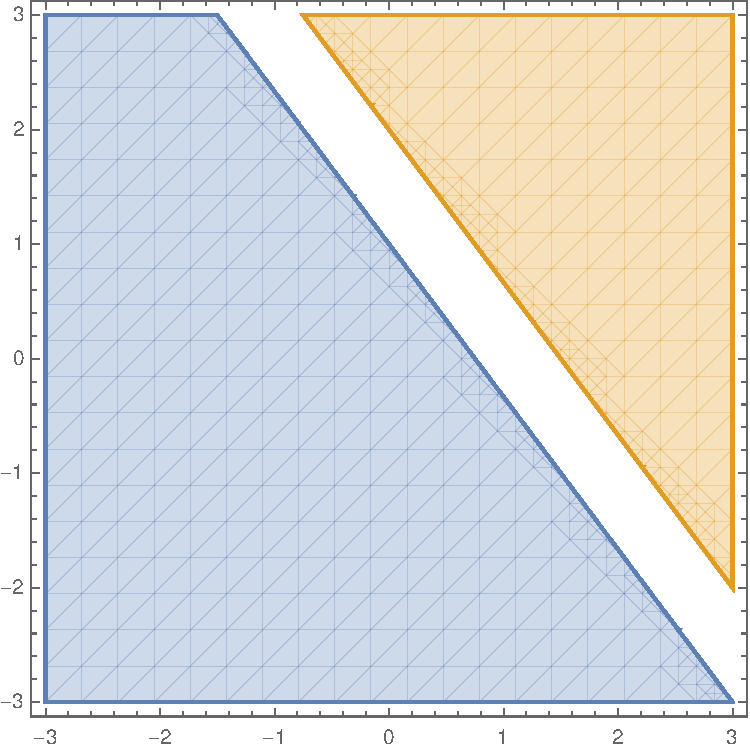
\includegraphics[width=\textwidth]{img/Axb.pdf}
        \caption{ \( Ax\leq b \) }
        \label{Axb}
    \end{subfigure}
    \hspace{.15\textwidth}
    \begin{subfigure}{.4\textwidth}\centering
        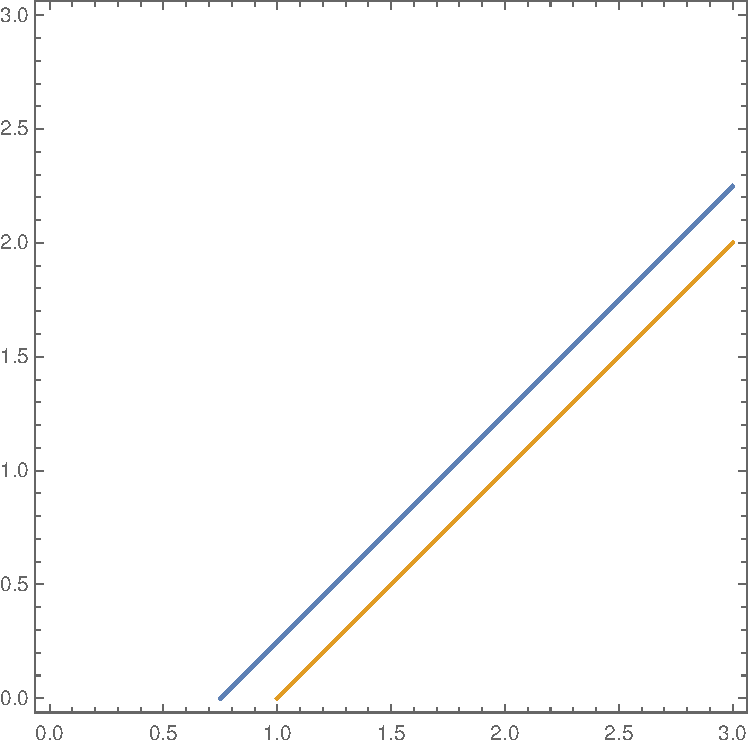
\includegraphics[width=\textwidth]{img/yAc.pdf}
        \caption{ \( y^TA = c^T \) }
        \label{yAc}
    \end{subfigure}
\end{figure}

\pagebreak
\end{solution}

\begin{problem}[Exercise 2.27]
    Let \( \tilde{x} \) be a feasible solution of \( \max\{c^Tx \st Ax\leq b\} \) and let \( \tilde{y} \) be a solution of \( \min\{y^Tb \st y\geq 0; y^TA=c^T \} \). Prove that \( \tilde{x} \) and \( \tilde{y} \) are the optimum solutions of the minimum and maximum, respectively if and only if for each \( i=1,2,\ldots,m \) one has: \( \tilde{y}_i=0 \) or \( a_i\tilde{x} = b_i \).    
\end{problem}

\begin{solution}

Denote the \( i \)-th row of \( A \) by \( a_i \).

First, note that if \( y \) is feasible, we have \( y^TA = c^T \) so that \( y^TAx = c^Tx \).

Second, note also that for any \( i=1,2,\ldots,m \), if \( x \) is feasible, we have \( a_ix\leq b \) so that \( a_ix-b \geq 0 \) and if \( y \) is feasible we have \( y_i\geq 0 \). Thus, \( y_i(a_ix-b) \geq 0 \).


We prove both directions at once. Indeed, suppose \( \tilde{x} \) and \( \tilde{y} \) are feasible. 

By duality, 
 \( \tilde{x} \) and \( \tilde{y} \) are the optimum solutions of the maximum and minimum respectively if and only if \( \tilde{y}^T b = c^T \tilde{x} \) which by the first note above is equivalent to,
\begin{align*}
    \tilde{y}^TAx = c^Tx = \tilde{y}^Tb 
\end{align*}

We can rearrange to find \( \tilde{y}^T(A\tilde{x}-b) = 0 \). Written in sum notation using the definition of matrix/vector multiplication we have,
\begin{align*}
    \sum_{i=1}^{m} \tilde{y}_i \left( a_i\tilde{x}-b \right) = 0
\end{align*}

Every term in this sum is non-negative by the second note above. Thus, the sum is zero if and only if each term is zero. That is, if and only if,
\begin{align*}
    y_i(a_i\tilde{x}-b) = 0 && \forall i=1,2,...,m
\end{align*}

Equivalently, for each \( i=1,2,...,m \) one has: \( \tilde{y}_i=0 \) or \( a_i\tilde{x} = b_i \). \qed
\end{solution}

\end{document}
